\chapter{Imágenes}

%las figuras son entornos flotantes, se colocarán donde mejor encajen en el documento final
\begin{figure}
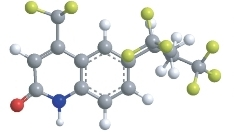
\includegraphics[width=3cm]{imagen.jpg}  %esta orden indica que ponemos aquí la imagen del fichero "imagen.jpg" con una anchura de 3cm; otros parámetros son scale, height...
\caption{Algo que encontré por %con esta orden determinamos el texto que acompaña a la figura
\href{http://www3.interscience.wiley.com/journal/13087/home/ForAuthors.html}{ahí.}%gracias al paquete hyperref, podemos poner enlaces a páginas en internet
}
\label{uno} 
\end{figure}

%las minipáginas son útiles para definir páginas más pequeñas dentro de otras; aquí aparecen dos una detrás de la otra, y la segunda empujada hacia la derecha por un \hfill
\begin{minipage}{8cm}
En la Figura \ref{uno} se puede ver una imagen. O bien podemos ponerla aquí a la derecha. 
\end{minipage} 
\hfill \begin{minipage}{3cm}
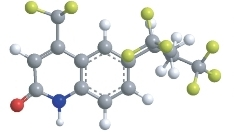
\includegraphics[width=2.5cm]{imagen.jpg}
\end{minipage}


